\section{引言}
\label{sec:introduction}

本文的研究对象是非中心对称钡--钇--锌硅酸盐$\mathrm{Ba_5Y_{12}Zn[O(SiO_4)]_8}$。研究目标有三点：确认目标相的组成与结构身份，厘清能够重复获得该相的成相条件，并判断含Zn相与无Zn四方Ba--Y硅酸盐之间是否存在连续的组成--结构关系。原始工作在开放体系中采用高温溶液法获得晶体，并以单晶X射线衍射确立结构\cite{ababaikeri2024ba5y12zn}。该结构同时具有高配位稀土--氧骨架和孤立或复合硅酸根单元，为复杂硅酸盐组装和非中心对称氧化物的组成设计提供了参照。

现有直接研究只回答了“晶体是否存在以及结构为何”，尚未给出可独立复现的投料组成、成相范围或批量相纯制备方法\cite{ababaikeri2024ba5y12zn}。因此，本文不试图从近邻化合物拼接出一条“最佳配方”，而是区分单晶生长、固相反应和相图筛查各自回答的问题，再据此设计能区分不同结构假设的实验。全文保留文献中的数值和限制条件；近邻体系仅用于提出实验参照。

\subsection{同类体系已有发现}

\paragraph{Ba--Y--Si--O四方谱系。}
早期助熔生长实验把$\mathrm{Ba_{5+x}Y_{13}Si_8O_{41}}$记录为伴生晶相。随后开展的151组BaO--K$_2$O--Y$_2$O$_3$--SiO$_2$--MoO$_3$实验表明，Y$_2$O$_3$/SiO$_2$比、MoO$_3$用量和冷却速率会改变硅酸盐的结构类型与晶体质量\cite{kolitsch2009crystal,wierzbickawieczorek2017high}。现代单晶研究把相关名义组成重审为非整比$\mathrm{Ba_xY_{26}Si_{16}O_{71+x}}$；陶瓷实验还发现，玛瑙研磨可能带入SiO$_2$，导致批量样品偏离名义配比\cite{yamane2024synthesis,yamane2024microstructure}。另一项相空间研究结合EDS、连续旋转电子衍射、同步辐射PXRD和中子衍射确认了$\mathrm{Ba_5Y_{13}[SiO_4]_8O_{8.5}}$，并观察到竞争相和玻璃区\cite{gulay2024navigation}。这些结果表明，目标相附近是由Ba/Y/Si比、氧计量、液相组成和热史共同控制的相区，而不是一条孤立配方。

\paragraph{Ba--Zn--Si--O结构近邻。}
Ba$M$SiO$_4$（$M=$Co、Zn、Mg）属于stuffed-tridymite衍生结构族，说明二价四面体阳离子可以在特定骨架中替换，但这不表示其结构与含Y目标相同型\cite{liu1993structures}。BaZn$_2$Si$_2$O$_7$的低温和高温结构可由中子与X射线衍射区分，说明观察温度和冷却路径会影响结构判定\cite{lin1999phase}。BaZnSi$_3$O$_8$的固相研究则依次采用煅烧、压片、烧结、受控冷却及同步辐射或实验室衍射\cite{zou2021crystal}。因此，Ba--Zn--Si--O文献的主要启示是同时记录Zn源、气氛、冷却路径以及高温和室温下的相组成，而不是直接移用某个温度。

\paragraph{Y--Si--O工艺近邻。}
Y$_2$SiO$_5$和Y$_2$Si$_2$O$_7$存在多种多型，已用高温溶液、熔体和Czochralski法制备。衍射、局域谱学与高温表征表明，不同多型及冷却后产物必须分别鉴定\cite{redhammer2003beta,becerro2004revisiting,dolan2008structures,pang2005study}。这些工作可帮助规范坩埚、助熔剂、挥发、慢冷和退火的记录，但不能证明$\mathrm{Ba_5Y_{12}Zn[O(SiO_4)]_8}$适用同样的生长方法。

\subsection{论文结构}

本文先核对目标相及相关结构的出处，再总结前人实验对组成、竞争相、污染和热史的认识，随后比较不同合成路线及其条件。最后提出局部相图、Zn--Y--氧计量耦合、固相与高温溶液并行以及Mg/Co类比四个研究方向。文中使用的两步无机逆合成模型只生成待验证的前驱体集合；温度、气氛、坩埚和表征方法仍依据文献和材料化学约束确定。

图~\ref{fig:research-roadmap}概括本文的论证路线。相关体系先用于确定结构关系、竞争相和工艺边界；相图与电荷平衡再提出候选组成，模型据此给出前驱体集合；固相成相和高温溶液长晶分别检验批量相区与单晶结构。根据相组成、实际化学计量和结构精修结果，逐轮调整组成和工艺。每轮实验均应至少排除一种结构或相区假设，而不是追求未经验证的“最佳配方”。

\begin{figure*}[t]
  \centering
  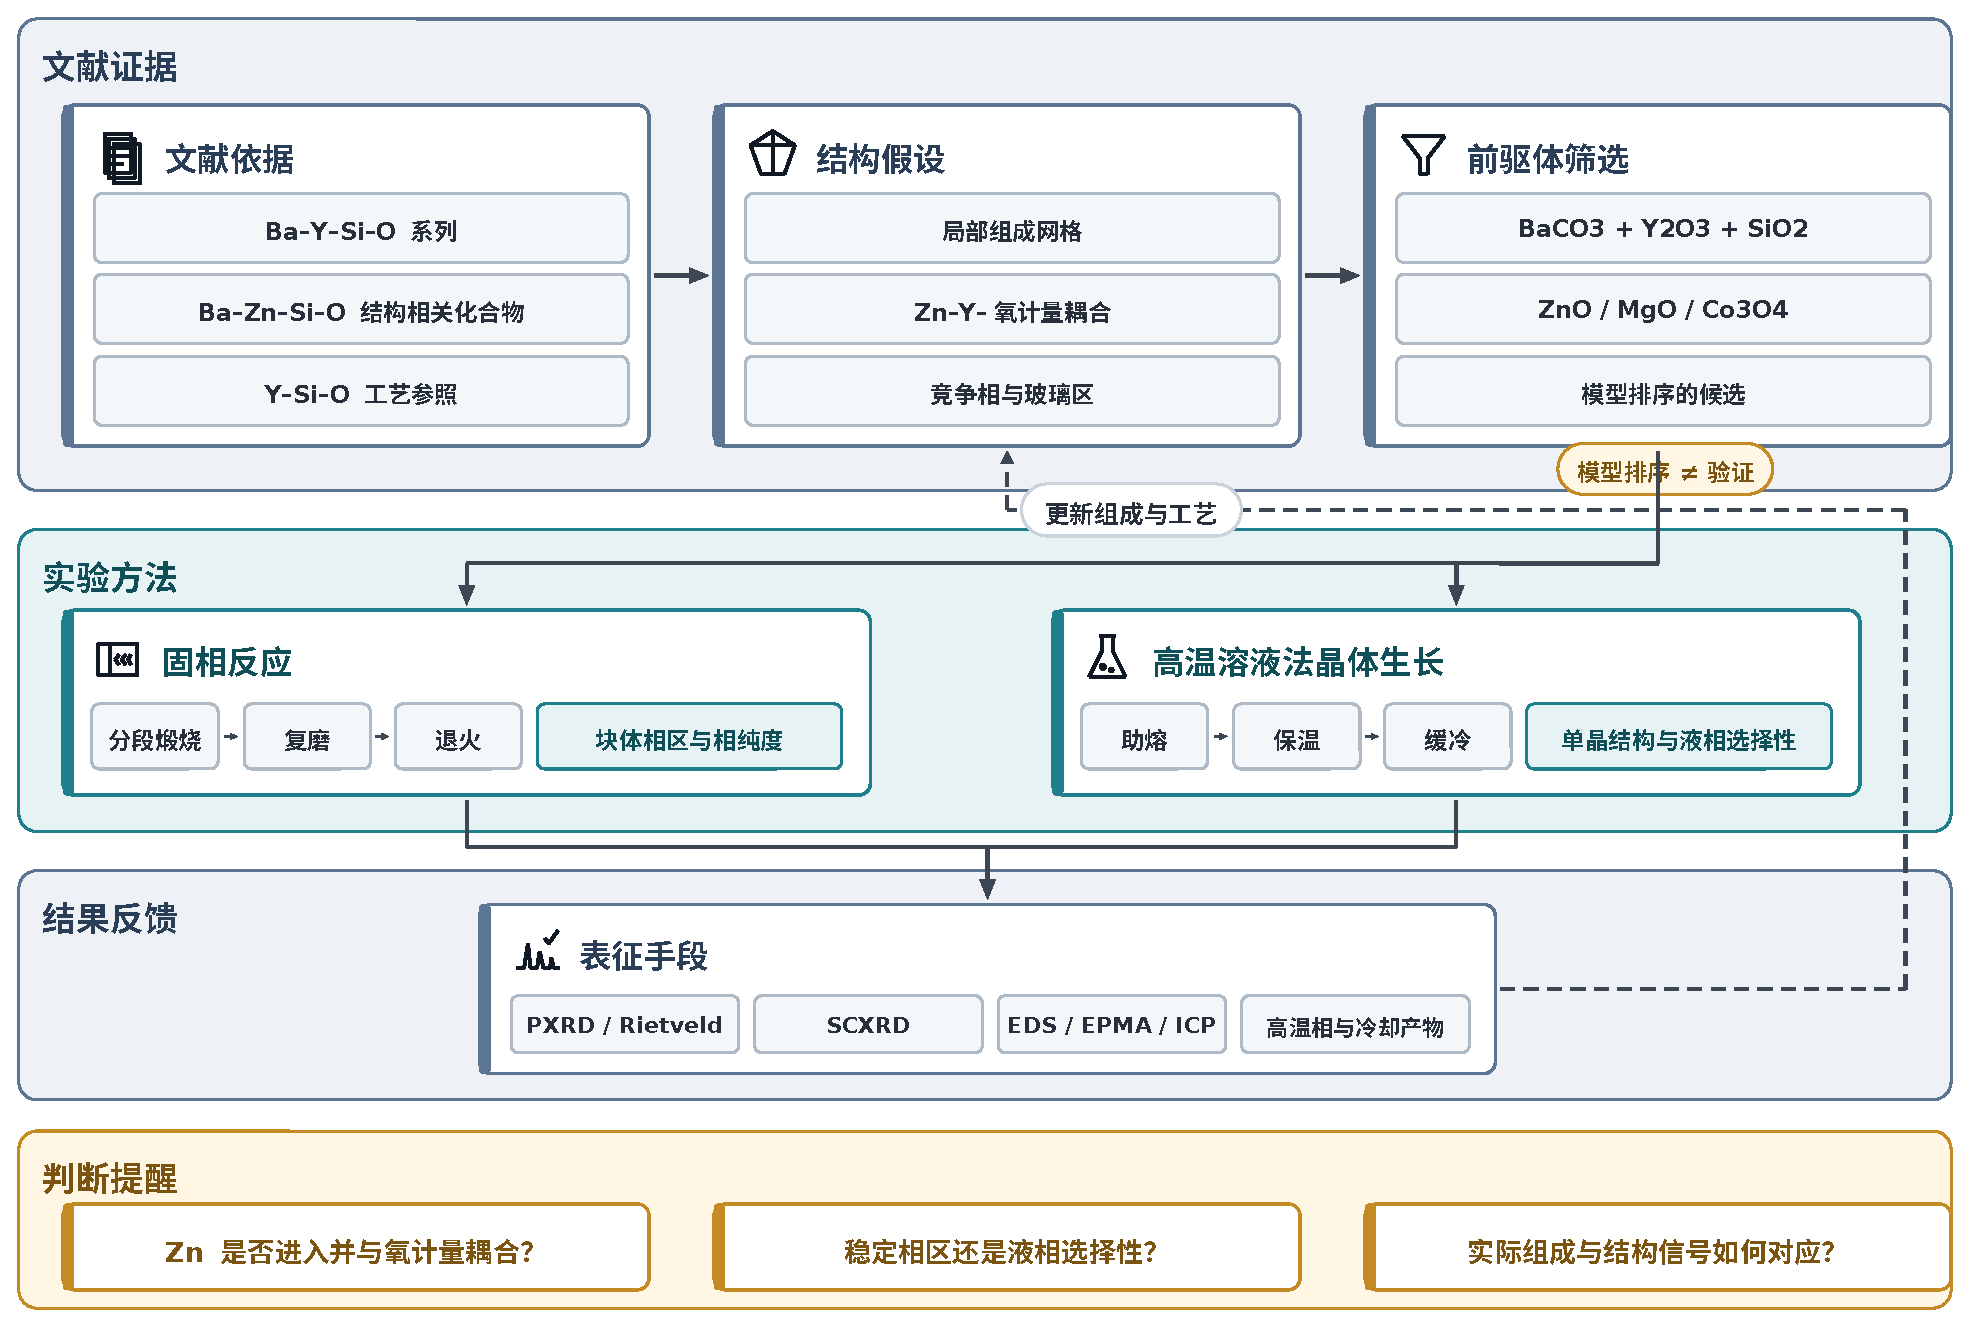
\includegraphics[width=\textwidth]{../figures/pdf/fig03_research_roadmap.pdf}
  \caption{本文的研究路线。Ba--Y--Si--O、Ba--Zn--Si--O和Y--Si--O体系先用于确定结构关系、竞争相和工艺边界；相图与电荷平衡提出候选组成，两步无机逆合成模型给出前驱体集合；固相成相与高温溶液长晶分别考察批量相区和单晶结构，表征结果用于调整后续组成和工艺。}
  \label{fig:research-roadmap}
\end{figure*}
